\graphicspath{{anexos/AnexoA-Formato-Planificacion-Inicial/recursos/}}

\section{Formatos de los Ficheros de Entrada} \label{Anexo:formato-planificacion-inicial}

El \autoref{capitulo:4}, concretamente en su \autoref{sec:4:req-io} recopila en forma de requisitos de software el formato que debe tomar los ficheros de entrada del sistema. En este anexo describimos en mayor profundidad dichos formatos, con ejemplos de cada uno de ellos.

Los ficheros de entrada se dividen en dos grupos, uno destinado a la información de la Dependencia o Unidad de Control concreta (por ejemplo, Palma, Barcelona, Madrid...) y otro destinado a la información específica del caso o instancia del problema.

Es importante destacar que todos los ficheros que describiremos a continuación emplean un formato CSV separado por punto y coma (;) en codificación UTF-8, que permite representarlo en forma de tablas.

\subsection{Ficheros de las Dependencias}

Encontramos un total de 4 ficheros, todos ellos obligatorios: en caso de no encontrarse uno de ellos, el sistema no podrá ejecutarse.

El primero de ellos, es la relación de sectores elementales, y deberá denominarse ``\texttt{ListaSectoresElementales\_Dependencia.csv}'' (donde \texttt{Dependencia} es el nombre de la Dependencia). Tiene la forma de la \autoref{fig:A:ejemplo-dependencias-sectores-elementales}. En caso de ser elemetal el propio sector, la columna correspondiente deberá estar vacía.

\begin{figure}[h]
	\centering
	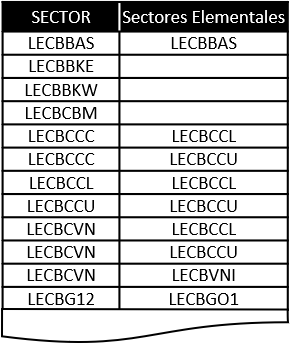
\includegraphics[width=0.5\linewidth]{ejemplo-dependencias-sectores-elementales}
	\caption{Fragmento del fichero \texttt{ListaSectoresElementales\_Barcelona.csv} como ejemplo del formato del fichero}
	\label{fig:A:ejemplo-dependencias-sectores-elementales}
\end{figure}

En segundo fichero es la matriz de afinidad de los sectores de la Unidad de Control. Es una matriz cuadrada de tamaño considerable, cuya primera fila y columna son iguales: la lista de los sectores en el mismo orden. Debe llamarse ``\texttt{MatrizAfinidad\_Dependencia.csv}''

\begin{figure}[h]
	\centering
	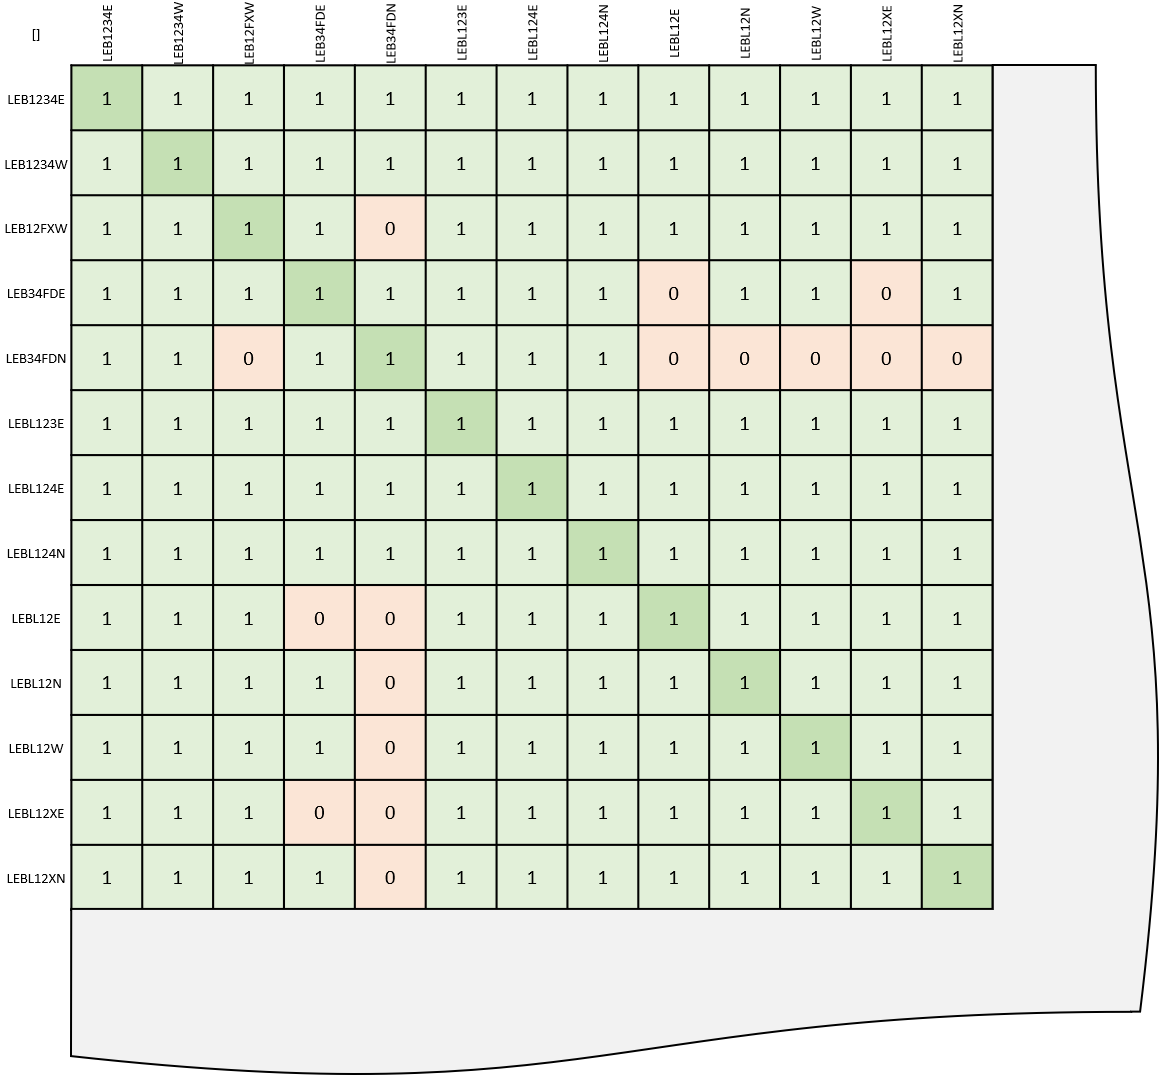
\includegraphics[width=\linewidth]{ejemplo-dependencias-matriz-afinidad}
	\caption{Fragmento de la Matriz de afinidad de Barcelona, tomada del fichero \texttt{MatrizAfinidad\_Barcelona.csv}}
	\label{fig:A:ejemplo-dependencias-matriz-afinidad}
\end{figure}

En caso de tomar valor 1, significa que los sectores son afines, mientras que si es 0, no lo son. Como puede verse, la diagonal principal siempre toma el valor de 1. Recuérdese que es un CSV, por lo que el fichero desde un editor de texto plano se verás así:

\noindent\fbox{%
	\parbox{\textwidth}{%
		[];L1234DXE;L1234DXN;L1234DXW;LEB1234E;LEB1234W;LEB12FXW; . . . \\
		L1234DXE;1;1;1;1;1;1;1;1;1;1;1;1;1; . . . \\
		L1234DXN;1;1;1;1;1;0;1;1;1;1;1;1;1; . . . \\
		L1234DXW;1;1;1;1;1;1;1;1;1;1;1;1;1; . . . \\
		LEB1234E;1;1;1;1;1;1;1;1;1;1;1;1;1; . . . \\
		LEB1234W;1;1;1;0;1;1;1;1;1;1;1;1;1; . . . \\
		LEB12FXW;1;1;1;1;1;1;1;0;1;1;1;1;1; . . . \\
		 . . . \\
	}%
}

El tercer fichero conforma la información que relaciona los sectores que pertenece a la Unidad de Control con los núcleos a los que pertenece cada uno de ellos. Además, incluye el tipo de sector, que puede ser ``RUTA'' o ``APP'' (aproximación). Debe llamarse ``\texttt{SectoresNucleos\_Dependencia}''. Véase un ejemplo en la \autoref{fig:A:ejemplo-dependencias-sectores-nucleos}

\begin{figure}[h]
	\centering
	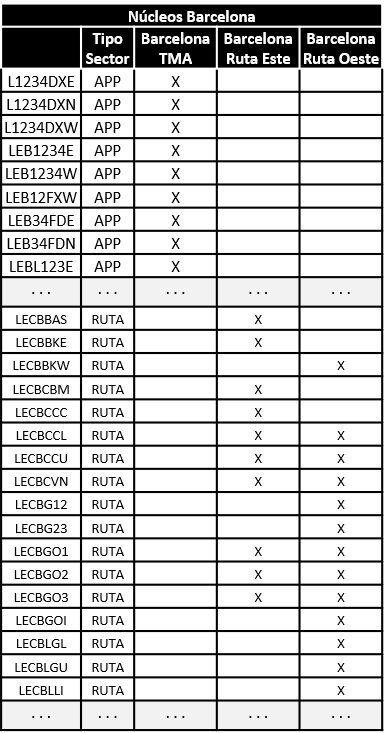
\includegraphics[width=0.5\linewidth]{ejemplo-dependencias-sectores-nucleos}
	\caption{Fragmento del fichero \texttt{SectoresNucleos\_Barcelona.csv}}
	\label{fig:A:ejemplo-dependencias-sectores-nucleos}
\end{figure}

El cuarto y último fichero relativo a las Dependencias tiene se denomina de la forma: \texttt{SectorizacionesSectoresVolumenes\_Dependencia.csv}'' y es aquel que recopila todas las configuraciones posibles de los sectores. Es aquí donde la cargamos al sistema la información que nos dice qué sectores pertenecen a la sectorización 3A, por ejemplo. Además, se ha de incluir más de una fila con la misma sectorización y el mismo sector, pero diferentes volúmenes para poder indicar cúales son los volúmenes que abarca un sector concreto. Por ejemplo, véase en la \autoref{fig:A:ejemplo-dependencias-sectorizaciones-sectores-volumenes} cómo la sectorización 1A y el sector LECBBKE aparecen 7 veces con un volumen distinto.

\begin{figure}[h]
	\centering
	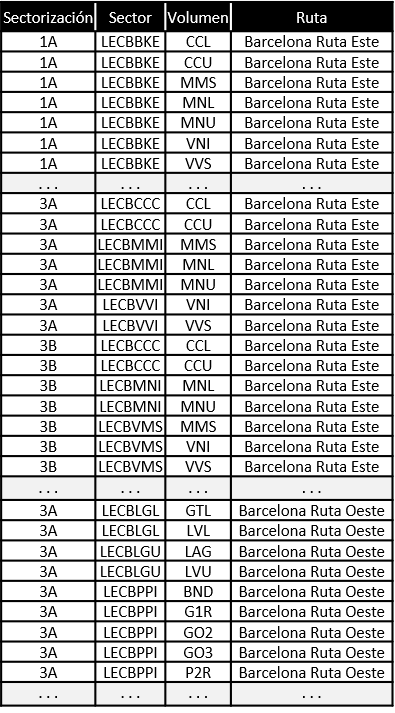
\includegraphics[width=0.6\linewidth]{ejemplo-dependencias-sectorizaciones-sectores-volumenes-reducida}
	\caption{Fragmento del fichero \texttt{SectorizacionesSectoresVolumenes\_Barcelona.csv}}
	\label{fig:A:ejemplo-dependencias-sectorizaciones-sectores-volumenes}
\end{figure}

Es importante destacar que no es lo mismo una sectorización para un núcleo u otro. Nótese en la figura anterior que los sectores que conforman una sectorización 3A para el núcleo ``Barcelona Ruta Este'' no son los mismos que aquellos indicados en el núcleo ``Barcelona Ruta Oeste''.

\subsection{Ficheros de los casos concretos}

Estos ficheros conforman los diferentes casos prueba del sistema, definidos en el \autoref{capitulo:5} y detallados el \autoref{Anexo:tabla-casos}. Cada caso tiene un identificador, el del Caso 1 empleado en este TFM es ``Id1m-01-01-2019'' y el nombre de cada fichero de entrada llevará al final su identificador.

El primero de los ficheros define el turno del caso: a qué hora comienza y termina y el tipo de turno, como puede verse en la \autoref{fig:A:ejemplo-casos-turno}.

\begin{figure}[h]
	\centering
	
\includegraphics[width=0.7\linewidth]{ejemplo-casos-turno}
	\caption{Fragmento del fichero \texttt{Turno\_Id1m-01-01-2019.csv}}
	\label{fig:A:ejemplo-casos-turno}
\end{figure}

Las siglas de los tipos de turnos son:

\begin{enumerate}[align=left]
	\item[M] Mañana
	\item[T] Tarde 
	\item[ML] Mañana Largo
	\item[MC] Mañana Corto
	\item[TL] Tarde Largo
	\item[TC] Tarde Corto
	\item[N] Noche
\end{enumerate}


El segundo de los ficheros define los intervalos en los que están abiertas cada sectorización. Como se muestra en la \autoref{fig:A:ejemplo-casos-sectorizaciones}, la aprtura de sectores puede indicarse con el nombre del sector o con una configuración, aunque lo más común es hacerlo mediante la configuración (CONF). Se requiere del núcleo en primera instancia, delimitando el espacio concreto que estamos definiendo. Tras el campo del tipo de información a leer del fichero, se indica si el o los sectores son de tipo nocturno (0 para false, 1 para verdadero), el nombre del sector o configuración según el tipo indicado y las hora de inicio y fin en las que dicha configuración se encuentra abierta.

\begin{figure}[h]
	\centering
	
\includegraphics[width=\linewidth]{ejemplo-casos-sectorizaciones}
	\caption{Fragmento del fichero \texttt{AperturaSectorizaciones\_Id1m-01-01-2019.csv}}
	\label{fig:A:ejemplo-casos-sectorizaciones}
\end{figure}

El tercer fichero describe los recursos humanos disponibles (los controladores) para cubrir las sectorizaciones indicadas en el fichero anterior. Se definen de la forma de la \autoref{fig:A:ejemplo-casos-controladores}. Como podemos ver, cada uno tiene un identificador, que debe ser único, y tiene dos tipos de acreditación, aquella que limita el tipo de sectores que puede controlar, y aquella que limita la zona del espacio aéreo que puede controlar (mediante núcleos).

\begin{figure}[h]
	\centering
	
\includegraphics[width=0.6\linewidth]{ejemplo-casos-controladores}
	\caption{Fragmento del fichero \texttt{RecursosDisponibles\_Id1m-01-01-2019.csv}}
	\label{fig:A:ejemplo-casos-controladores}
\end{figure}

Los dos siguientes ficheros permiten introducir en la entrada las incidencias, uno para las de tipo de cambio de sectorización respecto al inicial esperado y otro para altas y/o bajas de controladores.

El fichero destinado a la incidencia de tipo sectorización tiene el mismo formato que el segundo, representado en la \autoref{fig:A:ejemplo-casos-sectorizaciones}. Este fichero tendrá como nombre \texttt{ModificacionSectorizaciones\_Identificador.csv}.

El fichero destinado a la incidencia de altas y bajas de controladores tiene un formato similar al tercero, pero añadiendo una columna al principio, que permita definir si se trata de un alta o una baja, véase la \autoref{fig:A:ejemplo-casos-baja-alta}. El controlador de baja debe existir en el fichero de los recursos disponibles, mientras que el de alta debe ser un controlador nuevo. Por ello, en el caso de la baja, los datos del controlador (columnas ACREDITACIÓN, NÚCLEO y TURNO) son opcionales.

\begin{figure}[h]
	\centering
	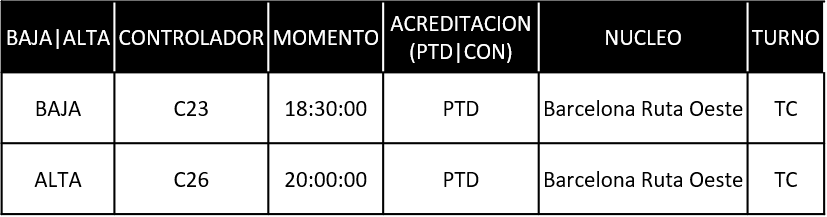
\includegraphics[width=0.8\linewidth]{ejemplo-casos-baja-alta}
	\caption{Fragmento del fichero \texttt{ModificacionRecursos\_Id6t-19-10-2018.csv} (Caso 7)}
	\label{fig:A:ejemplo-casos-baja-alta}
\end{figure}

Por último tenemos el fichero más importante: la planificación inicial del sistema, aquella que deja de ser válida debido a la contingencia acontecida. Este fichero se creó específicamente para este TFM y en un futuro, de cara al uso real de este sistema, deberá ser reemplazado por otro formato que sea común al del sistema que crea las planificaciones y que aquí llamamos \legacy{}. Este fichero fue creado lo más parecido posible al que emplean los trabajadores de los centros de control, que son de la forma de las Figuras \ref{fig:A:ejemplo-distribucion-crida-1} y \ref{fig:A:ejemplo-distribucion-crida-2}

\begin{figure}[h]
	\centering
	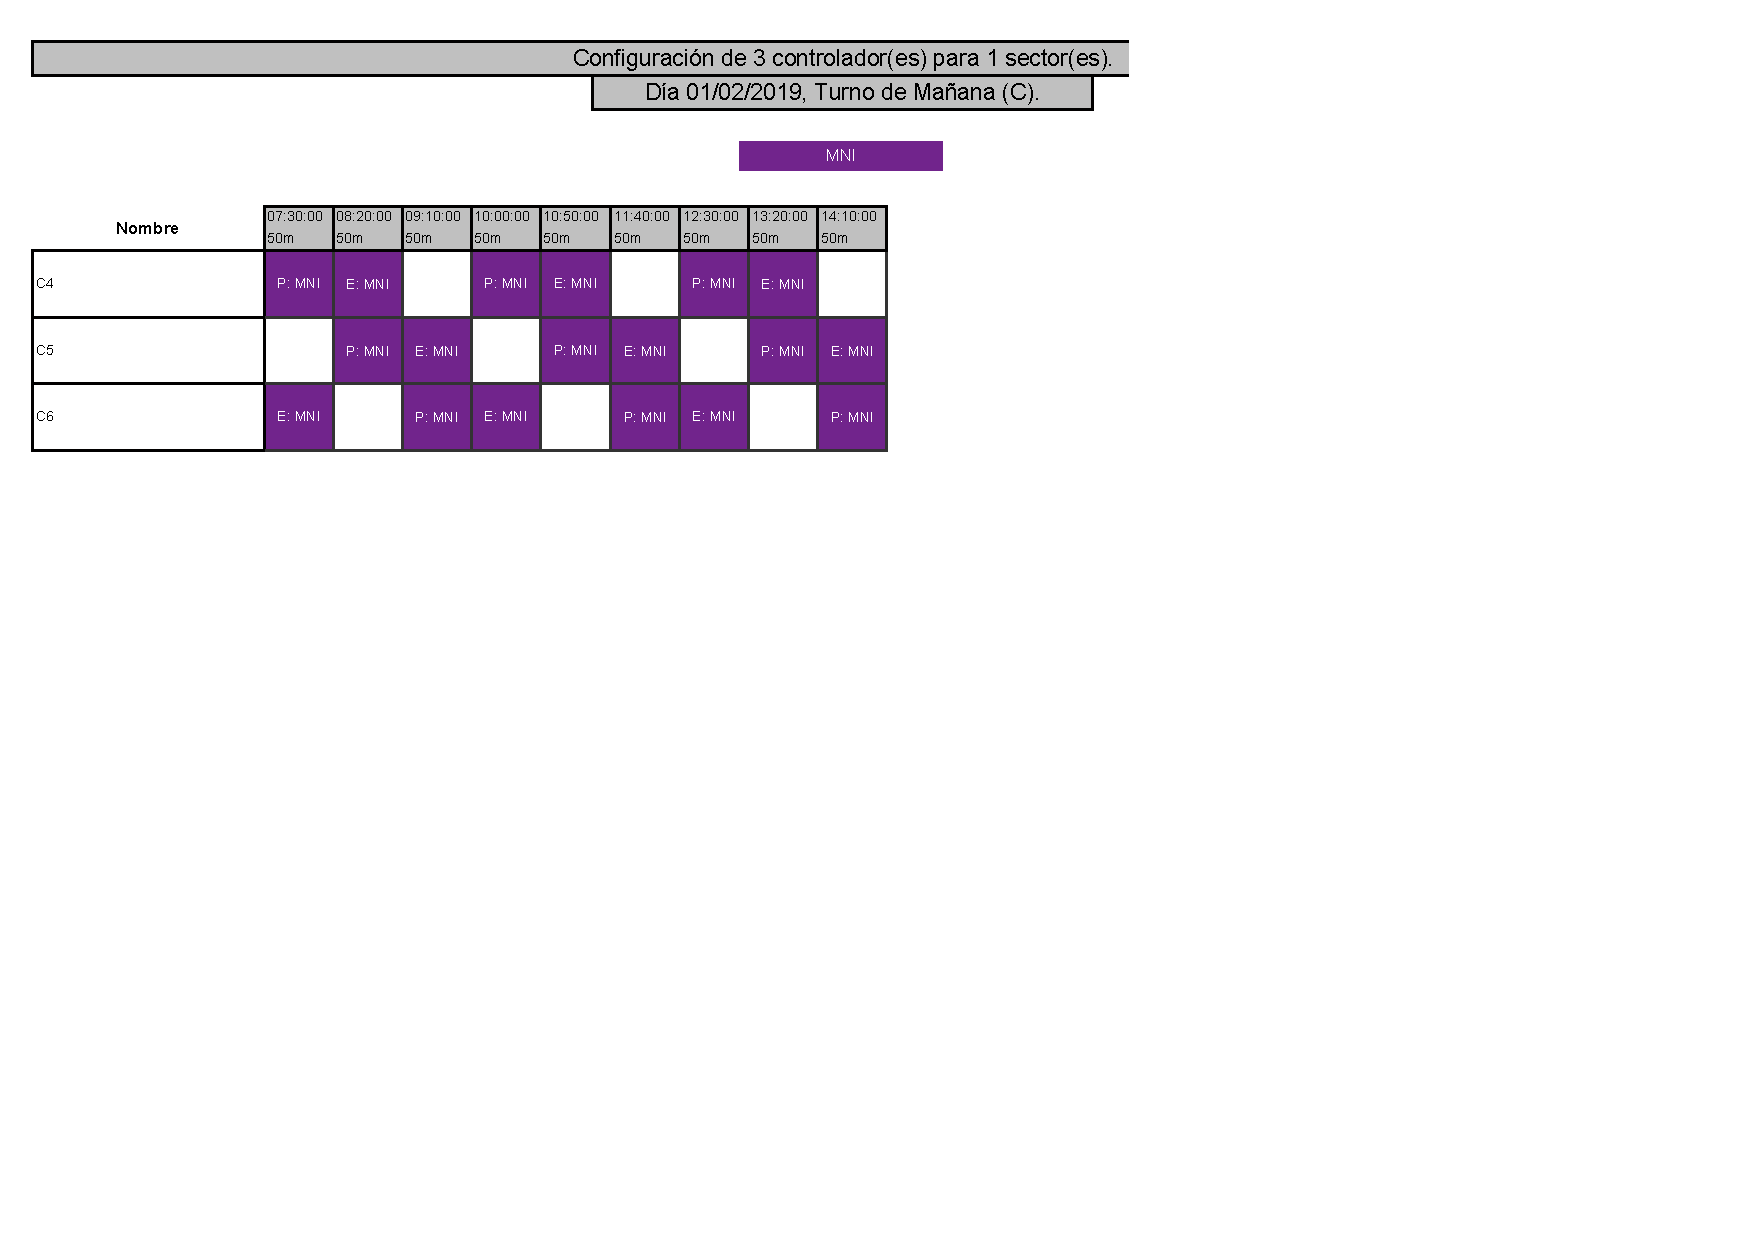
\includegraphics[width=\linewidth]{anexos/AnexoA-Formato-Planificacion-Inicial/recursos/ejemplo-distribucion-crida-1}
	\caption{Ejemplo de una de las planificaciones reales de CRIDA para el sector LECBMNI del Núcleo ESTE.}
	\label{fig:A:ejemplo-distribucion-crida-1}
\end{figure}

\begin{figure}[h]
	\centering
	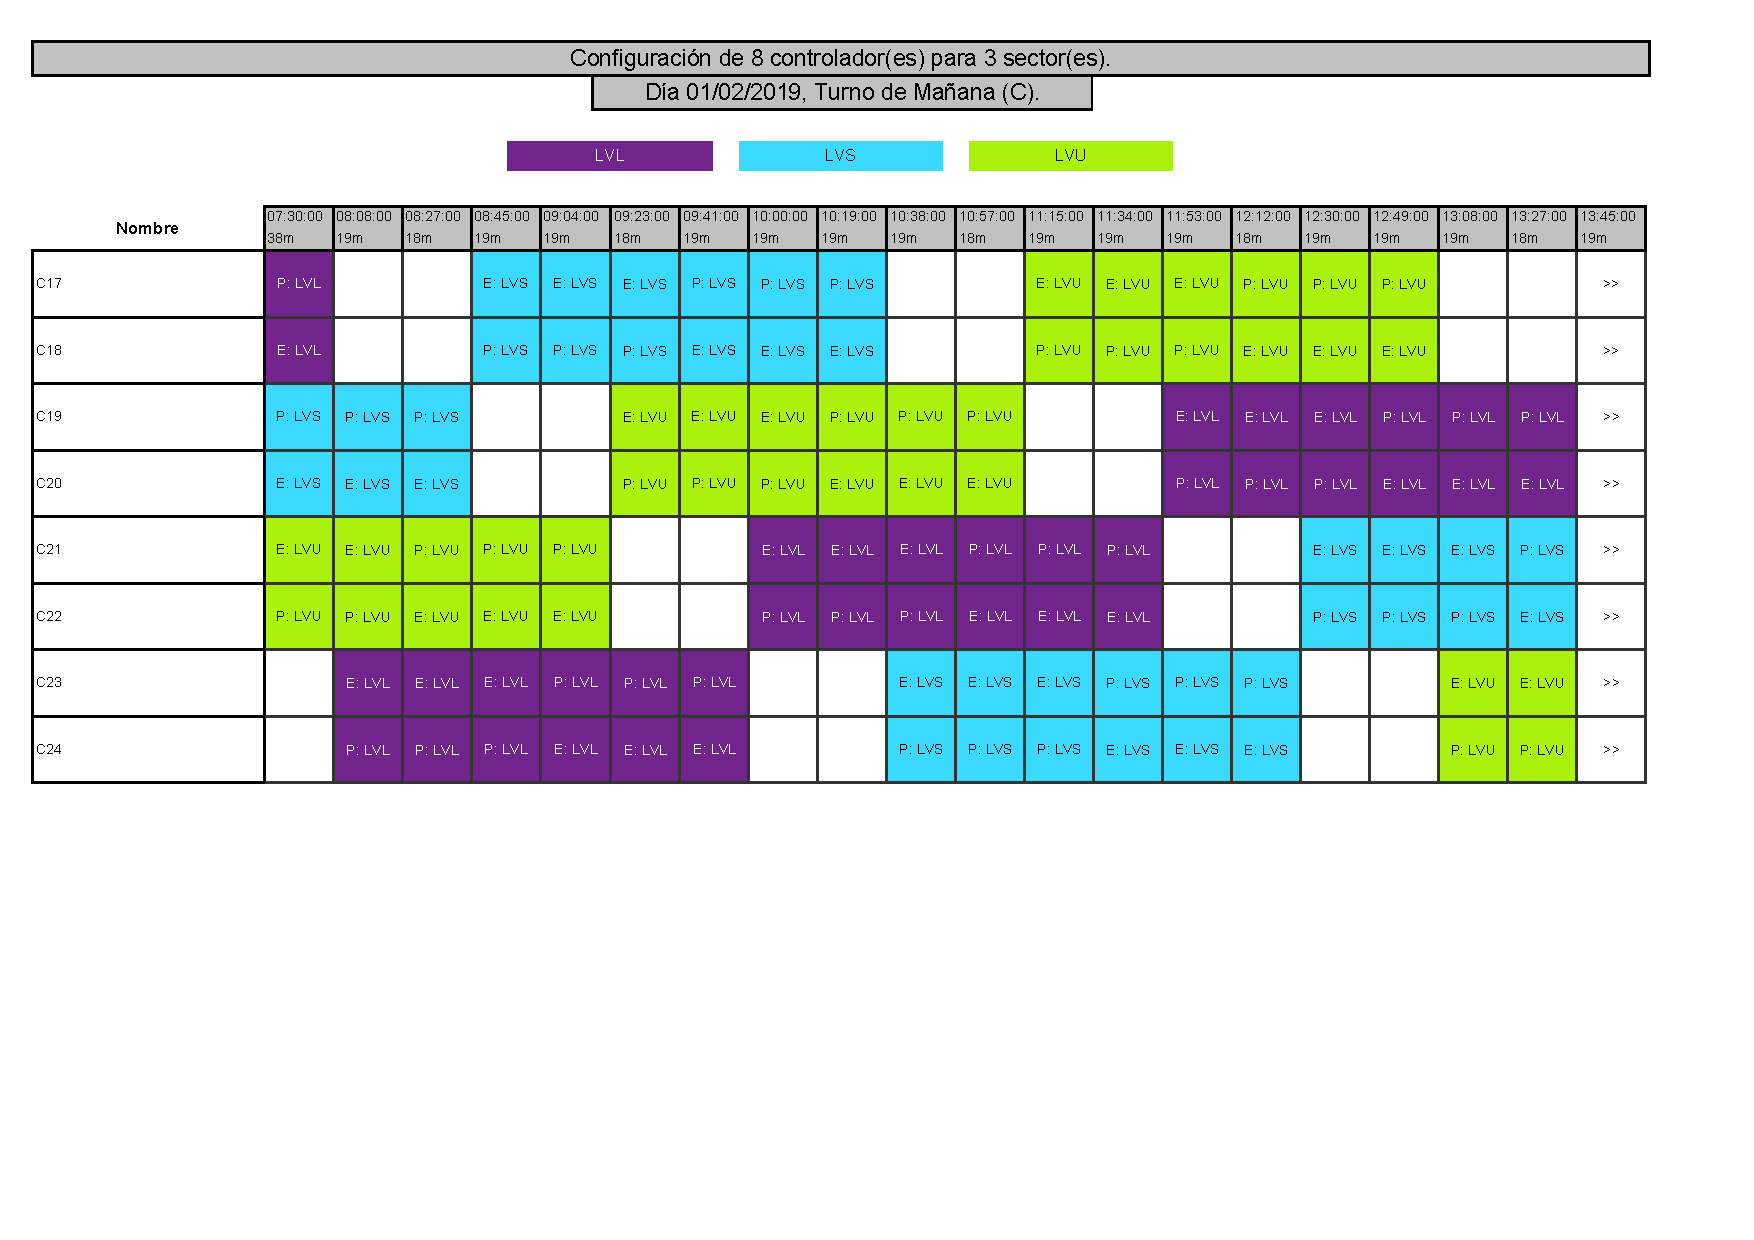
\includegraphics[width=\linewidth]{anexos/AnexoA-Formato-Planificacion-Inicial/recursos/ejemplo-distribucion-crida-2}
	\caption{Ejemplo de una de las planificaciones reales de CRIDA para los sectores LECBLVL, LECBLVS y LECBLVU del Núcleo OESTE.}
	\label{fig:A:ejemplo-distribucion-crida-2}
\end{figure}

Como puede verse se trata de, en el caso de la \autoref{fig:A:ejemplo-distribucion-crida-1}, una plantilla $3\times1$ (véase la \autoref{fig:3:plantilla-3x1} de la \autoref{sec:3:inicializacion-soluciones}); y en el caso de la \autoref{fig:A:ejemplo-distribucion-crida-2} una $8\times3$ (véase la \autoref{fig:6:plantilla8x3} de la \autoref{sec:6:trabajo-futuro}). Tiene la peculiaridad de que se indican los intervalos de hora en la cabecera de las tablas (en las figuras anteriores pueden verse 50m, 38m y 19m) en lugar de repetirse slot a slot como se venia haciendo en el formato de salida del sistema \legacy{}. 

Para pedir a CRIDA información de casos de prueba no podíamos emplear un formato slot a slot, pues sería costoso de crear de cara al personal de la organización. Lo mas sencillo fue replicar los estadillos anteriores en un solo fichero, de la forma de la figura adjunta al final del anexo. Dicha figura es autoexplicativa y fue la que se envió a CRIDA para que empleara como formato para enviarnos la información relativa a los casos de prueba. Podemos apreciar cómo las cabeceras (marcadas en color naranja pálido) tienen los números que en los estadillos de las figuras anteriores marcaban de forma equivalente, en ambos casos en minutos.

Por último se ha de notar que en este nuevo formato se ha de incluir todas las columnas de manera que la suma de los minutos de el total del tiempo del turno. Una limitación de la escalarización del tiempo en slots de 5 minutos (véase la \autoref{sec:3:representacion-soluciones}) es que los minutos que indiquemos en este fichero deben ser múltiplos de 5, por lo que la precisión del tiempo de la \autoref{fig:A:ejemplo-distribucion-crida-2} no es posible de codificar. En su lugar empleamos el múltiplo de 5 más cercano, procurando que la suma total siga siendo la misma, los 450 minutos que dura el turno. La figura adjunta no está completa, por eso aparecen unos puntos suspensivos al final del último estadillo, de lo contrario la imagen no cabría en este documento. El fichero con esta información se ha llamado \texttt{DistribucionInicial\_Identificador.csv}, siendo el del documento adjunto aquel empleado para el Caso 1.

\begin{landscape}
	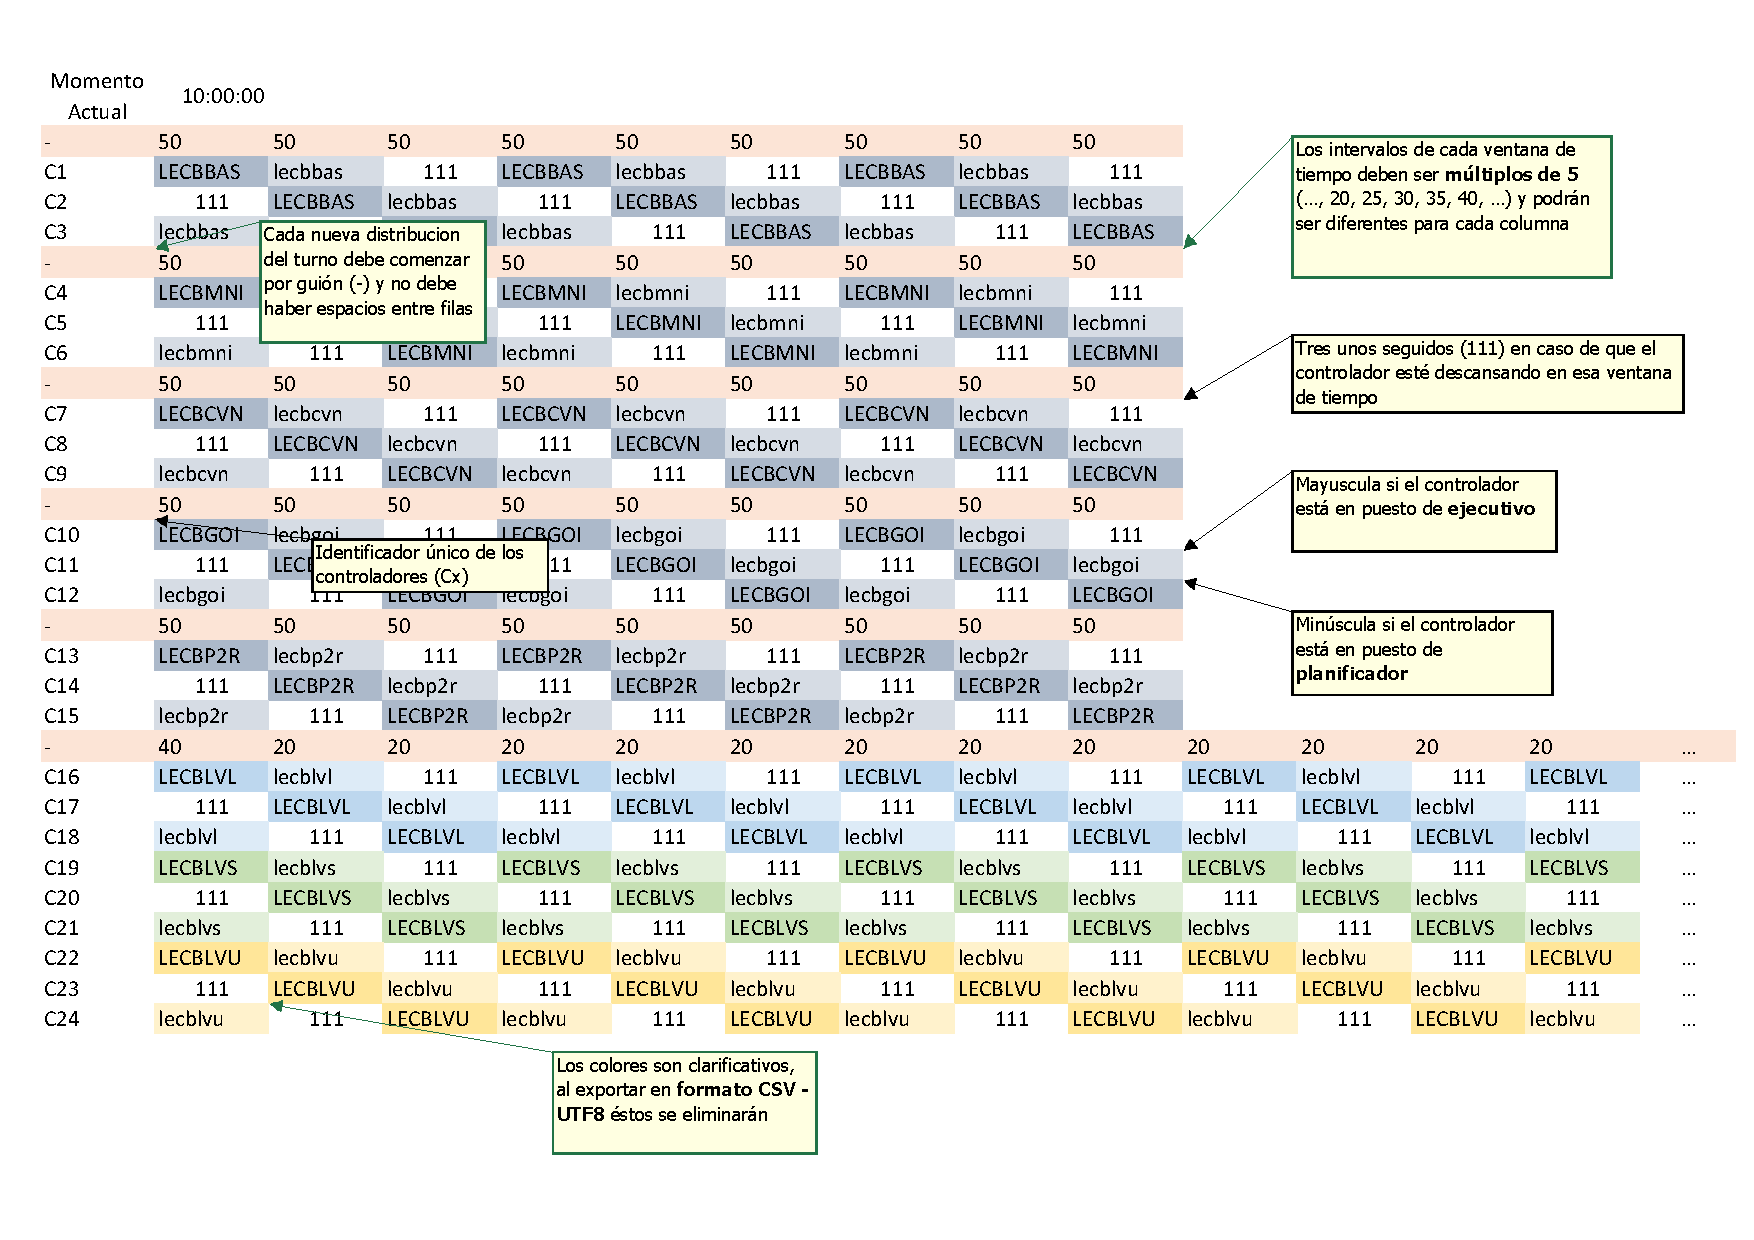
\includepdf[landscape=True]{DistribucionInicial}
\end{landscape}
